\chapter{Função Exponencial}
\section{Exponenciação}
\subsection{Definição}
\margem{A notação $a^n$ foi inventada por \textit{René Descartes}}
Algumas vezes desejamos multiplicar um número por ele mesmo várias vezes. Por exemplo, para calcular a área de um quadrado de lado $l$, nós usamos a seguinte fórmula: $$A = l.l$$Ou simplesmente$$A=l^2$$
O produto do mesmo número repetidas vezes é chamado de \textbf{exponenciação}. 
O número dois que aparece no canto superior direito de \textit{l} é o número que indica quantas vezes \textit{l} deve ser multiplicado por si mesmo. Este número é chamado de expoente.

\marginpar{
	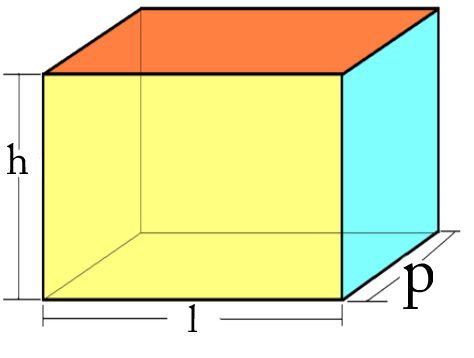
\includegraphics[width=0.85\marginparwidth]{imagens/cubo.png}
	\captionof{figure}{Paralelepípedo Reto-Retângulo}
	\label{fig:paralelepipedo}}
	
\exem{Aplicação na Geometria}{O volume de um \textit{paralelepípedo reto retângulo} (Figura \ref{fig:paralelepipedo}) é igual ao produto de sua altura ($h$), largura ($l$) e profundidade ($p$)$$V=h.l.p$$Chamamos de \textit{cubo} o \textit{paralelepipedo reto retângulo} que tem todos os lados iguais. Nesse caso $$V=l.l.l \Fl V=l^3$$}
\margem{Quando o expoente é $2$, dizemos que o número está elevado ao quadrado. Quando o expoente é $3$, dizemos que o número está elevado ao cubo.}

A exponenciação é amplamente utilizada nas ciências para descrever números muito grandes ou muito pequenos. A quantidade de moléculas de água em um copo de água é da ordem de $6.000.000.000.000.000.000.000.000$, ou $6.10^{24}$. Essa quantidade é praticamente incomensurável para nosso senso cotidiano: há mais moléculas de água em um copo de água do que copos de água no oceano!

Agora imagine que desejamos saber quantas moléculas de água existem no oceano e suponha que consiguimos estimar o número de copos de água no oceano em $10^{21}$. Assim: $\text{moléculas de água no oceano} = 6.10^{24} . 10^{21}$

Se desejamos obter o resultado, precisamos aprender a fazer cálculos com as exponenciações. Nosso primeiro conceito é que 
$$a^n = \underbrace{a.a\ldots a}_{n}$$
\margem{Poderíamos igualmente definir a multiplicação por $$a.n = \underbrace{a+a+\ldots+a}_{n}$$}

\label{def:exp_natural}\definicao{\textbf{Exponenciação} \\ \begin{center}

 Seja $a \in \R$, definimos $a^n$ por:
\end{center}
$$a^n = \begin{cases} a, & \text{ se } n=1 \\ a.a^{n-1}\ , &\text{ se } n >1 \end{cases}$$

\begin{center}
Na expressão $a^n$ chamamos $a$ de base e $n$ de expoente
\end{center}
}\\

A definição anterior é o que chamamos de \textit{definição por recorrência}. Para calcular $a^{10}$ precisamos antes saber quanto é $a^9$, para calcular $a^9$, precisamos saber quanto é $a^8$ e assim por diante. Esse tipo de definição é utilizada para evitar o uso das retiscências ($\ldots$), que não têm precisão matemática.
\begin{inlinexer}
Escreva uma definição por recorrência da multiplicação
\begin{flushright}
\tiny[\textbf{Solução}: Defina $a.n=a$, se $n=1$ e $a.n = a.(n-1) + a$, se $n>1$ ]
\end{flushright}
\end{inlinexer}
\exem{Cálculo de Algumas Potências}{\begin{enumerate}[a)]
\item $7^4 = 7.7.7.7 = 2401$
\item $(-4)^3 = (-4).(-4).(-4) = -64$
\item $(-4)^2 = (-4).(-4) = 16$ 
\item $\left (\frac{1}{3} \right)^3 = \frac{1}{3}.\frac{1}{3}.\frac{1}{3} = \frac{1}{27}$
\end{enumerate}
}
\margem{Repare que $(-4)^3$ é negativo e $(-4)^2$ é positivo.}
É importante salientar que a semelhança com a multiplicação não vai muito longe. Enquanto a multiplicação goza da propriedade comutativa ($a.b=b.a$), isso não acontece com a exponenciação. Ou seja, no geral $a^b \ne b^a$. Por exemplo:
\exem{$a^b \ne b^a$}{ $2^3 \ne 3^2$, afinal $2^3 = 2.2.2 = 8$ enquanto $3^2=3.3 = 9$.}
\newpage
\comecaexer
\subsection{Exercícios Elementares}
\begin{exer}Calcule utilizando a definição
\begin{enumerate}[a)]
	\item $2^2$
	\item $3^2$
	\item $-2^4$
	\item $(-2)^4$
	\item $-2^3$
	\item $(-2)^3$
	\item $2^5$
	\item $0,5^2$
	\item $1^2$
	\item $1^3$
	\item $0^1$
	\item $0^4$
	\item $(-1)^2$
	\item $(-1)^3$
	\item $(-1)^4$
	\item $-(-7)^2$
	\item $(-7)^2$
	\item $(2.3)^2$
	\item $2^2.3^2$
	\item $(4+1)^3$
	\item $4^3 + 1^3$
	\item $\left (\frac{2}{3}\right)^5$
	\item $\frac{2^5}{3^5}$
\end{enumerate}
\end{exer}
\begin{exer}[FUVEST](Modificado) - Calcule o valor da expressão $(0,2)^3+(0,16)^2$
\end{exer}
\begin{exer}Calcule a quantidade de algarismos dos seguintes números:
\begin{enumerate}[a)] 
	\item $10^4$
	\item $10^8$
	\item $10^n$, quando $n \in {\Z}^{+}_{*}$ Dica: Generalize o item a) e o item b)
	\item $352.10^8$
	\item $0,2.10^3$
	\item $200.10^{n+2}$
\end{enumerate}
\end{exer}
\begin{exer}Calcule o valor de $ab^2-a^3$ para $a = - \frac{x}{2}$ e $b=2x$
\end{exer}
\terminaexer\newpage\subsection{Complemento da Teoria}
Conforme pudemos observar nos exercícios, algumas vezes as exponenciações têm simplificações simples. As seguintes propriedades são válidas para todo $a \in \R$:
\caixaprop{
\begin{propriedade}\label{prop:exp_basico} $a^p \geq 0$, onde $p$ é um número par, ou seja, o resultado da exponenciação de qualquer número por um expoente par é sempre positivo, independente do sinal da base.
\end{propriedade}
\begin{propriedade}\label{prop:exp0}$0^n = 0$, para qualquer $n$ inteiro positivo.
\end{propriedade}
\begin{propriedade}$1^n=1$, para qualquer $n$ inteiro positivo.
\end{propriedade}
\begin{propriedade}$(-1)^i = -1$ e $(-1)^p = 1$, onde $i$ representa um inteiro positivo ímpar e $p$ representa um inteiro positivo par.
\end{propriedade}
\begin{propriedade} $(a.b)^n = a^n . b^n$
\end{propriedade} 
\begin{propriedade} $\left (\frac{a}{b}\right)^n = \frac{a^n}{b^n}$
\end{propriedade}
}

\textbf{Atenção}: $(a+b)^n \ne a^n+b^n$
\begin{inlinexer}
Calcule: $(-2)^3 + (-1)^2 + (-1)^{502} - 1^{55} + 0^1.(-5)^2$
\begin{flushright}
\tiny[\textbf{Solução}: $-8 + 1 + 1 -1 +0 = -7$]
\end{flushright}
\end{inlinexer}
\begin{exeresol} A esfera (Figura \ref{fig:esfera}) tem seu volume dado pela fórmula $V = \frac{4}{3} \pi r^3$, onde $r$ é o raio da esfera. Se duas esferas $a$ e $b$ são tais que seus raios são respectivamente $r_a$ e $r_b = 4r_a$, calcule a $\frac{V_a}{V_b}$, onde $V_a$ é o volume da esfera $a$ e $V_b$ é o volume da esfera $b$.
\end{exeresol}\textbf{Solução}\\
$$\frac{V_a}{V_b} = \frac{\frac{4}{3} \pi {r_a}^3}{\frac{4}{3} \pi {r_b}^3}$$
Simplificando: 
 $$\frac{V_a}{V_b} = \frac{{r_a}^3}{{r_b}^3} = \frac{{r_a}^3}{(4r_a)^3} = \frac{{r_a}^3}{4^3 {r_a}^3} = \frac{1}{64}$$
\marginpar{
 	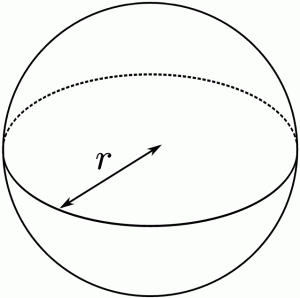
\includegraphics[width=0.8\marginparwidth]{imagens/esfera.png}
  \captionof{figure}{Esfera}
	\label{fig:esfera}}
\newpage
\section{Exponenciação (cont.)}
\subsection{Mais propriedades da exponenciação}
Nós aprendemos várias propriedades úteis para calcular a exponenciação de forma mais simples, sem precisarmos utilizar a definição por recorrência, que é longa e tediosa. Agora, veremos mais algumas propriedades que facilitam o cálculo da exponenciação. Antes, alguns exemplos:
\exem{Propriedades}{\begin{enumerate}[a)] \item $2^6 = \underbrace{2.2.2.2.2.2}_{6} = \underbrace{2.2.2}_{3}\underbrace{2.2.2}_{3}=2^3.2^3$
\item $5^{100} = \underbrace{5.5\ldots5}_{100} = \underbrace{5.5.5}_{3}.\underbrace{5.5\ldots5}_{97} = 5^3.5^{97}$
\item $(-2)^8 = \underbrace{(-2).(-2)\ldots(-2)}_{8} = \underbrace{(-2)(-2)(-2)(-2)}_{4}.\underbrace{(-2)(-2)(-2)(-2)}_{4}=(-2)^4.(-2)^4 = \left((-2)^4\right)^2$
\end{enumerate}
}\margem{Essas propriedades vão nortear a nossa definição da exponenciação quando o expoente for negativo ou uma fração!\\As demonstrações estão no apêndice.}
\caixaprop{\begin{propriedade}\label{prop:expsoma}
$a^{m+n}=a^m.a^n$
\end{propriedade}
\begin{propriedade}\label{prop:expprod}
$a^{m.n}=(a^m)^n$
\end{propriedade}
}\\
Vamos explorar um pouco a propriedade \ref{prop:expsoma}. Conforme os exemplos anteriores, vimos que $$5^{100}=5^3.5^{97}$$Isso também pode ser escrito da seguinte forma:$$5^{97}=\frac{5^{100}}{5^3}$$Assim, podemos escrever mais uma propriedade:
\caixaprop{\begin{propriedade}\label{prop:expdiferenca}
$a^{m-n} = \frac{a^m}{a^n}$, Para $a \ne 0$
\end{propriedade}
}
\begin{inlinexer}
Simplifique: $\frac{(a^4.b^5)^2}{(a.b)^3}$
\begin{flushright}
\tiny[\textbf{Solução}: $\frac{a^8.b^{10}}{a^3.b^3}=\frac{a^8}{a^3}\frac{b^{10}}{b^3}=a^5.b^7$]
\end{flushright}
\end{inlinexer}
\begin{inlinexer}[EsPCEx-Modificado] Efetuando-se $k^{p+1}:(-k^{1-2p})$, o que se obtem?
\begin{flushright}
\footnotesize[\textbf{Solução}: $-\frac{k^{p+1}}{k^{1-2p}} = -k^{p+1 -(1-2p)}$ $=-k^{3p}$]
\end{flushright}
\end{inlinexer}
\subsection{Expoentes Inteiros Negativos}
Com as propriedades desenvolvidas até aqui estamos prontos para extender a nossa definição de exponenciação e englobar expoentes inteiros. Porém, devemos salientar, que com essa extensão virão restrições: até agora pudemos fazer a exponenciação para qualquer base, independentemente de ser positiva, negativa ou nula. Ao introduzirmos expoentes negativos vamos excluir a possibilidade da base nula. Nós já veremos o porquê.
\margem{$0^0$ é uma forma indeterminada. Isso vem da óbvia contradição entre a propriedade \ref{prop:exp0} e a definição \ref{def:exp_inteira}. Frequentemente utilizamos $0^0=1$ para efeitos de simplificação.}
Seguindo as propriedades anteriores, vamos definir $a^0$, para $a\ne0$. Para isso, tome $m=1$ e $n=1$ na Propriedade \ref{prop:expdiferenca}. Isso nos dá:$$a^{1-1}=\frac{a^1}{a^1} \Fl a^0=1$$Agora, vamos calcular $a^{-1}$. Tome $m=0$ e $n=1$, com isso:$$a^{0-1}=\frac{a^0}{a^1} \Fl a^{-1}=\frac{1}{a}$$E finalmente, para um número inteiro negativo qualquer, vamos utilizar a Propriedade \ref{prop:expprod}. Tome $n=-1$ $$a^{m.(-1)} = (a^m)^{-1} \Fl a^{-m} = \frac{1}{a^m}$$Com essas considerações, a única forma consistente de definir a exponenciação para expoentes inteiros é a que se segue:
\margem{Para frações também vale: $\left ( \frac{a}{b}\right)^{-n} = \left(\frac{b}{a}\right)^n$ }
\definicao{\label{def:exp_inteira}\textbf{Exponenciação de Inteiros Não Positivos}\\ \begin{center}
Seja $a \in R_*$, definimos: 
\end{center}
$$a^n = \begin{cases} 1, &\text{ Se } n = 0 \\ \frac{1}{a^{-n}}, &\text{ Se } n<0 \end{cases}$$
}\\
Os expoentes negativos são muito utilizados para descrever grandezas muito pequenas. O sistema internacinal de unidades possui vários prefixos de unidades que são potências negativas de 10. Por exemplo, um miligrama são $10^{-3}$ gramas. Um mililitro são $10^{-3}$ litros e assim por diante (veja a tabela \ref{tab:prefixosSI}).
\margem{
\captionof{table}{Prefixos do SI}\label{tab:prefixosSI}
\begin{tabular}{|l|l|l|}
  \hline
  Prefixo & Símbolo & Potência \\
  \hline
  deci & d & $10^{-1}$\\
  centi & c & $10^{-2}$\\
  mili & m & $10^{-3}$\\
  micro & $\mu$ & $10^{-6}$\\
  nano & n & $10^{-9}$\\
  pico & p & $10^{-12}$\\
  \hline
\end{tabular}
}
\newpage
\comecaexer
\subsection*{Exercícios Elementares}
Atenção! Não se esqueça de utilizar as propriedades vistas na aula passada!
\begin{exer}Calcule
\begin{enumerate}[a)]
\item $2^{-1}$
\item $2^{-2}$
\item $-2^{-1}$
\item $-2^{-2}$
\item $(-3)^{-6}$
\item $\frapar{1}{5}^{-3}$
\item $-\frapar{3}{2}^{-2} $
\item $\left(-\frac{3}{5} \right)^{-4}$
\item $(0,125)^{-2}$
\item $\frac{1}{3^{-2}}$
\end{enumerate}
\end{exer}
\begin{exer} Se $\pi^2 \approx 10$, calcule $\pi^4$ e $\pi^6$
\end{exer}
\begin{exer} Calcule $\left ( \frac{2^0 + 2^4 + 2 - 2^3}{2^{-1}+2{-1}} \right)^2$
\end{exer}
\begin{exer}
Quanto devemos somar a $(-2)^{-1}$ para obter $(-2)^2$?
\end{exer}
\begin{exer} Classifique em (V) ou (F)
\begin{enumerate}[a)]
\item $(2^4)^3 = 4^6$
\item $\frac{2^3+2^2}{3.2^2} = 3^{-1}+3^{-1}+3^{-1}$
\item $(x+y)^{-2} = x^{-2}+y^{-2}$ Para qualquer $x,y \in \Rep$
\item $2^{-1}-3^{-1}=6^{-1}$
\item $\frac{1}{x^{-2}} = x^2$ Para qualquer $x \in \Rep$
\item $(a^b)^c = a^{(b^c)}$ Para quaisquers $a,b,c \in \Rep$
\end{enumerate}
\end{exer}
\begin{exer}[PM]Calcule $\left(\frac{2}{3}-1\right)^2+2(-1)^3$
\end{exer}
\begin{exer}[PM]Calcule $2^{-1}\frac{1}{2^5}$
\end{exer}
\begin{exer}[CN-Modificado]
Calcular: $\frapar{3}{7}^{-2} + \frac{5}{2}(7)^{-1} + \frapar{1}{4}^{-2}$
\end{exer}\margem{Dica: $0,43535\ldots = \frac{431}{990}$}
\begin{exer}[CN] Resolver a expressão $\frac{\frac{2}{3}+1}{\frac{4}{3}-1}-\frapar{\frac{2}{3}-2}{3-\frac{1}{2}}^0 + \frac{1}{2^{-1}} + 0,43535\ldots$
\end{exer}
\begin{exer}
Simplifique $\frac{5^{2n+1} - 25^n}{5^{4n}}$
\end{exer}
\begin{exer}
Simplifique $\frac{2^5 - 2^4}{3} + \frapar{1}{2}^{-1} + 0,125^{-3} + 0,25^{-2}$
\end{exer}
\begin{exer}Calcule o inverso da expressão:
$\frac{\left( \frac{3}{4}+\frac{2}{3}\right)\frac{1}{2} + \frac{0,5}{0,001}3.10^{-2}}{\frac{5}{4}}$
\end{exer}
\begin{exer}
Calcule n na expressão abaixo: $$\frac{4^5+4^5+4^5+4^5}{3^5+3^5+3^5}\ \frac{5.6^5+6^5}{2^5+2^5} = 2^n $$
\end{exer}
\begin{exer}[CN]Na expressão abaixo $a$ e $b$ são números inteiros e positivos. Calcule $a+b$. $$\frac{(0,125)^{b-a}}{8^{a-b}}+21\frapar{b}{a}^0+a^b=191$$
\end{exer}
\terminaexer
\newpage
\section{Raízes Enésimas e Expoentes Racionais}
\subsection{Função Inversa da Exponencial}
Algumas vezes precisamos responder perguntas do tipo \textit{qual potência de $2$ é $64$?} e também do tipo \textit{qual número elevado a $2$ é $64$?}. Essas duas perguntas geram respostas e operações inversas muito diferentes. Antes de começarmos a explorar o conceito de exponenciação para expoentes racionais, vamos ver formas de definir a operação inversa da exponenciação. O problema surge da \textit{não comutatividade} da exponenciação. Ou seja, dados dois números $a$ e $b$ podemos fazer duas perguntas: \margem{Escreveremos o $x$ da primeira equação, quando existir como $x = \log_{a}b$}
\begin{enumerate}[1)] 
\item Qual potência de $a$ é igual a $b$? ($a^x=b$)
\item Qual número elevado a $a$ é igual a $b$? ($x^a=b$)
\end{enumerate}
\margem{Na multiplicação teríamos a mesma resposta para as duas perguntas: $x = \frac{b}{a}$}
\exem{Titulo}{Se tomarmos $a=2$ e $b=64$ teremos duas equações: $$2^x=64 (\text{ solução : }x=6)$$ $$x^2=64 (\text{ solução : }x=8 \text{ ou } x=-8)$$}Por enquanto, vamos nos concentrar em responder a segunda pergunta.
\subsection{Raízes Enésimas}
Nessa seção nos concentraremos na pergunta: Dado um número qualquer $b$ e um expoente inteiro $a$, é sempre possível encontrar uma base $x$ tal que $x^a=b$? "\\Para respondermos essa pergunta, fixe $a \in \mathbb{Z}$ e seja $$f\colon \R \to \R$$ $$x \mapsto x^a$$Queremos então encontrar $x$ que satisfaça $f(x)=b$. Se essa função não for inversível podemos ter mais de uma resposta ou nenhuma.
\marginpar{
	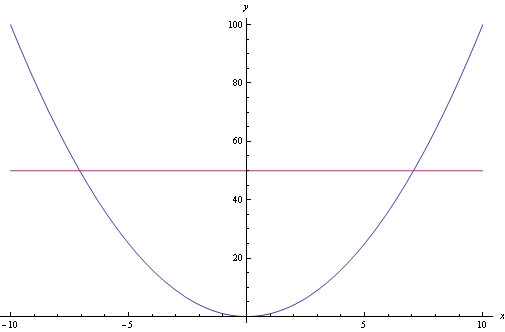
\includegraphics[width=0.85\marginparwidth]{imagens/xquadrado.png}
	\captionof{figure}{Gráfico de $y=x^2$}
	\label{fig:xquadrado}}
\begin{inlinexer}Seja $f(x)=x^2$ (veja a Figura \ref{fig:xquadrado}). Discuta se é possível definir a inversa de $f$ e sob quais restrições.
\begin{flushright}
\footnotesize[\textbf{Solução}: Uma possível solução é tomar $\mathbb{D}(f)=\Rep$ e $\mathbb{CD}(f)=\Rep$, tornando a função bijetora e, logo, inversível]
\end{flushright}
\end{inlinexer}
Vamos estudar dois casos distintos: \begin{enumerate}[1)]
\item $f(x)=x^a$ e $a$ é par
\item $f(x)=x^a$ e $a$ é ímpar
\end{enumerate}
Quando o expoente é par, vimos na Propriedade \ref{prop:exp_basico} que o resultado é sempre positivo. Assim a imagem da função vai ser estritamente positiva e ela não será injetora em todos os números reais (porque $f(a)=f(-a)$)
\marginpar{
	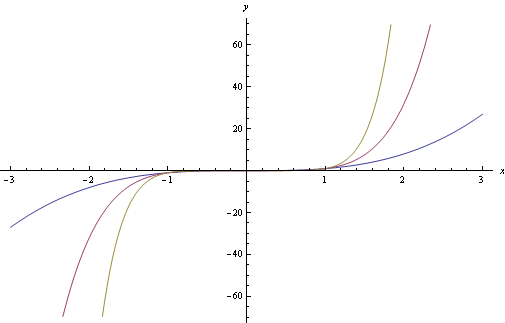
\includegraphics[width=\marginparwidth]{imagens/ximpar.png}
	\captionof{figure}{Gráficos de $y=x^3, y=x^5, y=x^7$}
	\label{fig:ximpar}
	}

\exem{Titulo}{Seja $f\colon \R \to \R$ tal que $x\mapsto x^6$. Então $$f(-x)=(-x)^6=(-1)^6.x^6 = x^6=f(x)$$ e portanto $f$ não é injetora, não sendo também inversível.}
\margem{A palavra raiz é utilizada há muitos séculos com o sentido aqui definido. Sua origem é \textit{radix}, do latim: lado. Raiz quadrada significaria, originalmente, \textit{o lado do quadrado}. Assim o lado do quadrado de área 9 é 3, ou, como dizemos \textit{raiz quadrada} de 9 é 3.}

Prova-se utilizando o princípio da indução finita que quando $a$ é ímpar, $f$ é inversível (veja a Figura \ref{fig:ximpar}). Da discussão segue dois resultados importantes \begin{enumerate}[I -] 
\item Quando $a$ é par, $f(x)=x^a$ só é inversível se limitarmos domínio e contra-domínio.
\item Quando $a$ é ímpar, $f(x)=x^a$ é inversível em todo $\R$.
\end{enumerate}

Isso nos leva a seguinte definição:
\margem{Poderíamos também definir $\sqrt[n]{a}$ como a menor raiz da equação. Algebricamente tudo continuaria consistente, mas perderíamos o sentido histórico da \textit{raiz quadrada} }
\definicao{\label{def:raiz_n}\textbf{Raiz Enésima} \\ \begin{center} Seja $a \in \R$ $$\sqrt[n]{a} \text{ é a maior raiz real da equação
 } x^n=a \text{, caso exista}$$ $a$ é chamado de radicando e $n$ de índice. \end{center}
 } 
 \margem{
Por que $1024=2^{10}$? É a fatoração!

\begin{tabular}{l|l}
  1024 & 2\\
  \hline
  512 & 2\\
  256 & 2\\
  128 & 2\\
  64 & 2\\
  32 & 2\\
  16 & 2\\
  8 & 2\\
  4 & 2\\
  2 & 2 \\
  1 & $1024 = 2^{10}$\\
  \end{tabular}
}
 \exem{Titulo}{\begin{enumerate}[a)]
 \item $\sqrt[3]{64}=4$, pois $4^3=64$
 \item $\sqrt[2]{36} = 6$, pois $6^2 =36$. Embora $(-6)^2=36$ temos que $6>(-6)$
 \item $\sqrt[n]{0} = 0$, pois $0^n=0$
 \item $\sqrt[n]{1} = 1$, pois $1^n=1$
 \item Não existe $\sqrt[2]{-1}$, pois não existe $x^2=-1$ em $\R$
 \item $\sqrt[10]{1024} = 2$, pois $2^{10}=1024$. Embora $(-2)^{10}=1024$, $2>-2$
 \item $\sqrt[n]{x^n} = x$, se $n$ for ímpar. 
 
 \end{enumerate}}
 
 As raízes enésimas observam as seguintes propriedades:
 \caixaprop{Para $a,b \in \Rep$
 \begin{propriedade}\label{prop:raizvezes}
 $$\sqrt[n]{ab}=\sqrt[n]{a}\sqrt[n]{b}$$
  \end{propriedade} 
  \begin{propriedade}\label{prop:raizdivide}
  $$\sqrt[n]{\frac{a}{b}} = \frac{\sqrt[n]{a}}{\sqrt[n]{b}}$$
  \end{propriedade}
  \begin{propriedade}\label{prop:raizexpoente}
  $$ \left ( \sqrt[n]{a} \right)^m = \sqrt[n]{a^m}$$
  \end{propriedade}
  \begin{propriedade}\label{prop:raizindices}
  $$\sqrt[n]{\sqrt[m]{a}}=\sqrt[n.m]{a}$$
  \end{propriedade}
  \begin{propriedade}\label{prop:raizcortaindice}
  $$\sqrt[kn]{a^k}=\sqrt[n]{a}$$
  \end{propriedade}
  \begin{propriedade}\label{prop:raizmonotona}
  $$\sqrt[n]{a}<\sqrt[n]{b} \Fl a < b$$
  \end{propriedade}
  
}
 \margem{Tome cuidado ao aplicar as propriedades! $$1 =\sqrt{(-1)^2}\ne \left ( \sqrt{-1} \right)^2$$Afinal de contas $\sqrt{-1} \notin \R$}
 \exem{Titulo}{Para simplificarmos $\sqrt{18}$ primeiro fatoramos $18=2.3^2$ assim $$\sqrt{18}=\sqrt{3^2.2}\stackrel{P. \ref{prop:raizvezes}}{=}\sqrt{3^2}\sqrt{2}=3\sqrt{2}$$}
 \begin{exeresol}
 Coloque em ordem crescente: $\sqrt{2}$, $\sqrt[4]{15}$, $\sqrt[3]{10}$
 
 
  \textbf{Solução:} Primeiro precisamos colocar as raízes no mesmo índice. O mmc entre $2,4$ e $3$ é $12$. Colocando todas as raízes no mesmo índice (Propriedade \ref{prop:raizcortaindice}) temos $$\sqrt[12]{2^6}, \sqrt[12]{15^3}, \sqrt[12]{10^4}$$ $$\sqrt[12]{64},\sqrt[12]{3375},\sqrt[12]{1000}$$Assim, pela Propriedade \ref{prop:raizmonotona}: $\sqrt{2}<\sqrt[3]{10}<\sqrt[4]{15}$
\end{exeresol} 
\margem{Racionalizar significa eliminar os radicais do denominador}

\begin{exeresol}
Racionalize: $\frac{1}{\sqrt{3}},\frac{1}{\sqrt{2}+\sqrt{3}}, \frac{1}{\sqrt{3}-\sqrt{2}}$


 \textbf{Solução:} $\frac{1}{\sqrt{3}} = \frac{1}{\sqrt{3}} \frac{\sqrt{3}}{\sqrt{3}}=\frac{\sqrt{3}}{\sqrt{3}\sqrt{3}} = \frac{\sqrt{3}}{3}$
 
 $\frac{1}{\sqrt{2}+\sqrt{3}} = \frac{1}{\sqrt{2}+\sqrt{3}} \frac{\sqrt{2}-\sqrt{3}}{\sqrt{2}-\sqrt{3}} = \frac{\sqrt{2}-\sqrt{3}}{(\sqrt{2}+\sqrt{3})(\sqrt{2}-\sqrt{3})} = \frac{\sqrt{2}-\sqrt{3}}{2-3}=\frac{\sqrt{2}-\sqrt{3}}{-1}= -(\sqrt{2}-\sqrt{3}) = \sqrt{3}-\sqrt{2}$
 
 $\frac{1}{\sqrt{3}-\sqrt{2}}= \frac{1}{\sqrt{3}-\sqrt{2}}\frac{\sqrt{3}+\sqrt{2}}{\sqrt{3}+\sqrt{2}} = \frac{\sqrt{3}+\sqrt{2}}{(\sqrt{3}-\sqrt{2})(\sqrt{3}+\sqrt{2})}=\frac{\sqrt{3}+\sqrt{2}}{3-2}=\sqrt{3}+\sqrt{2}$
 \end{exeresol}

\subsection{Radicais Duplos} 
Uma curiosidade sobre radicais: É possível que dois radicais com formas diferentes correspondam ao mesmo número:
\exem{Titulo}{$\sqrt{8 + \sqrt{15}} = \frac{\sqrt{2}}{2} \left(\sqrt{15}+1\right)$ pois ambos os lados quando elevados ao quadrado resultam em $8 + \sqrt{15}$. Como são ambos positivos, necessariamente, são iguais}
\inlinexer{Sejam $A,B \in \mathbb{Q}^+$ tais que $\sqrt{A^2-B} \in \mathbb{Q}$. Então, escreva $\sqrt{A+\sqrt{B}}$ como a soma de dois radicais simples

\begin{flushright}
\tiny[\textbf{Solução}: Se $\sqrt{A+\sqrt{B}}=\sqrt{x}+\sqrt{y}$ então $A+ \sqrt{B} = x + y + 2\sqrt{xy}$ Logo $A = x+y$ e $B=4xy$. Isolando $y$ temos $A = x + \frac{B}{4x}$ assim $4xA = 4x^2 + B$ logo $x = \frac{A + \sqrt{A^2 -B}}{2}$ e $y = \frac{A-\sqrt{A^2-B}}{2}$]
\end{flushright}

}
\begin{exeresol}[EPCAR] Transformar $\sqrt{7+4\sqrt{3}}$


 \textbf{Solução} Usando o exercício anterior temos $A=7$ e $B=3.4^2$ (porque a expressão anterior é $\sqrt{A+\sqrt{B}})$. Verificando, temos que $A^2-B = 49-48=1$ é um quadrado perfeito, assim podemos escrever $$\sqrt{7+4\sqrt{3}}= \sqrt{\frac{7+\sqrt{1}}{2}} + \sqrt{\frac{7-\sqrt{1}}{2}}=\sqrt{4} + \sqrt{6} = 2 + \sqrt{6}$$
\end{exeresol}

Como ressaltamos anteriormente o \textit{radical duplo} é uma curiosidade, assim como a \textit{racionalização}. Apesar da grande quantidade de exercícios não é uma parte essencial para o entendimento da matéria e nem conceitualmente complicada, sendo um exercício técnico e tedioso diferente dos exercícios que utilizam habilidades matemáticas de fato.

\subsection{Irracionalidade de algumas raízes}
Tendo estabelecido via função inversa a existência das raízes quadradas e enésimas no geral, estamos aptos a apresentar concretamente números irracionais. O que é feito nessa seção é a demonstração clássica de que $\sqrt{2} \notin \mathbb{Q}$
\caixaprop{
\begin{teorema}[Irracionalidade de $\sqrt{2}$] $\sqrt{2} \notin \mathbb{Q}$
\begin{proof}
Suponha por absurdo que $\sqrt{2} \in \mathbb{Q}$. Então existe uma fração $\frac{p}{q}$ irredutível (mdc($p,q$)$=1$) de números inteiros tal que $x = \frac{p}{q}$. Logo $$\left(\frac{p}{q}\right)^2= 2$$ $$p^2 = 2q^2$$Logo $p^2$ é par. A única possibilidade para $p^2$ ser par é se $p$ também o for (caso contrário, se $p$ for ímpar, $p^2$ também o será). Assim $p=2k$. Substituindo teremos: $$(2k)^2=2q^2$$ $$q^2=2k^2$$Assim $q^2$ também é par e, logo, $q$ é par. Assim $2 | p$ e $2 | q$ e $2 | $mdc($p,q$) contrariando a hipótese de que mdc($p,q$)$=1$.
\end{proof}
\end{teorema}
}
\margem{Corre a lenda no folclore matemático de que o primeiro homem que descobriu que não havia nenhuma proporção de números inteiros  cujo quadrado fosse dois sofreu uma morte misteriosa por ação dos pitagóricos.\\ A escola pitagórica defendia que a natureza era composta por números e os \textit{irracionais} não tinham espaço nessa filosofia. }


Na verdade a raiz quadrada de um número positivo que não é quadrado perfeito é sempre irracional. Embora seja um resultado simples exige um conhecimento mínimo de teoria dos números e não será feito aqui.
\inlinexer{Prove que $\sqrt{3}$ é irracional
\begin{flushright}
\footnotesize[\textbf{Solução}: Se $\left(\frac{p}{q}\right)=3$ então $p^2=3q^2$ e logo $3|p^2 \Fl 3|p$. Logo $p=3k$ assim $3k^2=q^2$ e $3|q$ de onde mdc($p,q$)$\geq3$ ]
\end{flushright}
}
\subsection{Expoentes Racionais}
Estamos aptos agora a definir os expoentes racionais. Vamos manter em mente a Propriedade \ref{prop:expsoma} e tentar definir $a^\frac{p}{q}$ de forma a respeitá-la. Observe que: $$\left(a^\frac{p}{q}\right)^q = a^p$$ Dessa forma, de acordo com a Definição \ref{def:raiz_n} $$a^\frac{p}{q} = \sqrt[q]{a^p}$$Assim a única forma natural de definirmos a exponenciação para expoentes racionais é: 
\definicao{\label{def:exporacional}\textbf{Expoente Racional} \\ \begin{center} Seja $a \in \R$  e $p,q \in \mathbb{Z}$ com $q \ne 0$ e mdc($p,q$)$=1$ então $$a^\frac{p}{q} = \sqrt[q]{a^p}$$Se $a<0$ então $q$ deve ser ímpar.\end{center}}
\exem{Exemplos de Expoentes Racionais}{
\begin{enumerate}[a)]
\item $32^\frac{2}{5} = \sqrt[5]{32^2} = \left(\sqrt[5]{32}\right)^2 = 2^2=4$
\item $27^\frac{5}{3} = \left(\sqrt[3]{27}\right)^5 = 3^5=243$
\item $8^{-0,333\ldots}=8^\frac{-1}{3}=\left(\sqrt[3]{8}\right)^{-1}=\frac{1}{2}$
\item $0,0625^{0,5} = 0,0625^\frac{1}{2} = \sqrt{0,0625}=\sqrt{\frac{1}{16}}=\frac{1}{4}$

\end{enumerate}
}
\comecaexer
\subsection*{Exercícios Elementares}
\subsubsection{Raízes}
\begin{exer}Classifique como (V) ou (F) \begin{enumerate}[a)]
\item $\sqrt{100}=10$
\item $\sqrt{4} = \sqrt{-4}$
\item $\sqrt{36} = \pm 6$
\item $\sqrt{x^2} = x$
\item $\sqrt{x^4}=x^2$
\item $\sqrt[n]{\sqrt[m]{x}}=\sqrt[nm]{x}$
\item $\sqrt[3]{0.125} = \sqrt{0.25}$
\item $\sqrt{x^14} =x^\frac{1}{7}$
\item $-\sqrt{49}=-7$
\end{enumerate}
\end{exer}
\begin{exer}[EPCAR-Mod.]Simplifique, $7\sqrt{32} - 5\sqrt{2} +\sqrt{8}$
\end{exer}
\begin{exer} Simplifique e se possível resolva
\begin{enumerate}[a)]
\item $\sqrt{45}$
\item $\sqrt{175}$
\item $\sqrt{169}$
\item $\sqrt{675}$
\item $\sqrt[3]{-675}$
\item $\sqrt[5]{\pi^{10}}$
\item $\sqrt{27}$
\item $\sqrt{100}$
\item $\sqrt[4]{81^{-1}}$
\end{enumerate}
\end{exer}

\begin{exer} Prove que $f \colon \R \to \R$ dada por $f(x)=x^3$ é uma função crescente e, logo, injetora.
\end{exer}

\begin{exer} Simplifique
\begin{enumerate}[a)]
\item $(\sqrt{8} + \sqrt{2})\sqrt{32}$
\item $\sqrt{50} + \sqrt{18} + \sqrt{98}$
\item $\sqrt{3000} + \sqrt{300}+ \sqrt{30}+ \sqrt{3}$
\item $\sqrt{76x^4}$
\item $(\sqrt[3]{16}+4\sqrt[3]{3})^2$
\item $\sqrt{\frac{5}{4}} \colon \sqrt{\frac{2}{3}}$
\item $\frac{\sqrt[3]{3}}{\sqrt[2]{2}}$
\end{enumerate}
\end{exer}
\begin{exer}[EsPCEx]Reduzir à expressão mais simples: $$ \sqrt{\frac{a\sqrt{b}}{\sqrt[3]{ab}}}.\sqrt[4]{b}$$
\end{exer}
\begin{exer}[EsPCEx]A expressão $\frac{3\sqrt{a}}{\sqrt[4]{a}}$, é igual a:
\begin{enumerate}[A ( )]
\item $3a$
\item $3$
\item $\sqrt{a}$
\item $3 \sqrt[4]{a}$
\item n.d.a
\end{enumerate}
\end{exer}

\begin{exer}[PM] Efetuando: $\left( \sqrt[3]{\sqrt{64}}\right)^2$ tem-se:
\begin{enumerate}[A ( )]
\item $2$
\item $4$
\item $8$
\item $12$
\item $16$
\end{enumerate}
\end{exer}

\begin{exer}[EsPCEx] A expressão $\sqrt{3} + \sqrt{12} -\sqrt{27} +\sqrt{867}$, é igual a:
\begin{enumerate}[A ( )]
\item $17\sqrt{3}$
\item $3\sqrt{95}$
\item $0$
\item $3\sqrt{17}$
\item n.d.a
\end{enumerate}
\end{exer}
\begin{exer}[EPCAR - Mod.] Escreva em ordem crescente $\sqrt{3}$, $\sqrt[4]{5}$ e $\sqrt[3]{4}$.
\end{exer}
\begin{exer}[EsPCEx]A soma, $\sqrt[3]{a} + \sqrt[4]{a}$ é:
\begin{enumerate}[A ( )]
\item $\sqrt[7]{2a}$
\item $\sqrt[7]{a}$
\item $\sqrt[12]{a^7}$
\item $\sqrt[12]{a^3+a^4}$
\item n.d.a.
\end{enumerate}
\end{exer}
\begin{exer}[EPCAR] Se $\frac{\sqrt{5}+\sqrt{2}}{\sqrt{5}}=K(\sqrt{10}+5)$, então $K$ é igual a:
\begin{enumerate}[A ( )]
\item $\frac{\sqrt{5}}{5}$
\item $5$
\item $\frac{1}{5}$
\item $5\sqrt{2}$
\item $\frac{\sqrt{2}}{2}$
\end{enumerate}
\end{exer}
\begin{exer}[EsPCEx]Substituir pelo sinal correspondente $$(\sqrt{3}-1)^2=\ldots(1-\sqrt{3})^2 $$
\end{exer}
\begin{exer}[EsPCEx]Calcular a expressão $(3+2\sqrt{5})^2-(3\sqrt{3}-2\sqrt{5})^2+(3\sqrt{2})^2-\sqrt{720}+\sqrt{2160}$
\end{exer}
\begin{exer}[EsPCEx]Efetuar as operações: $ 6a\sqrt{63ab^3}-3\sqrt{112a^3b^3}+2ab\sqrt{343ab}-5b\sqrt{28a^3b} $
\end{exer}
\begin{exer}[EsPCEx]Efetue:$$\sqrt[5]{a\sqrt[3]{a^2}}.\sqrt[6]{\sqrt[4]{a^9}}.\sqrt[3]{a^2\sqrt[8]{a^7}}$$
\end{exer}
\begin{exer}[CN]Simplificar a expressão: $$\sqrt{16x^3y} - \sqrt{25xy^3}-(x-5y)\sqrt{xy}$$
\end{exer}
\begin{exer}[CN]Simplificar e efetuar: $$3\sqrt[3]{a^4b^4} + 5a\sqrt[3]{b^4} + b\sqrt[3]{a^4b} $$
\end{exer}
\begin{exer}[EPCAR] Calcular o valor da expressão $\frac{2\sqrt[6]{27}}{\sqrt[4]{9}}$
\end{exer}
\begin{exer}[CN]Efetuar $\sqrt{24}\sqrt[4]{36}$
\end{exer}
\begin{exer}[CN]Efetuar $\sqrt{200}\sqrt[3]{108}$
\end{exer}
\begin{exer}[CN]Dê a expressão mais simples de: $$\frac{\frac{\sqrt[4]{a}}{\sqrt[6]{a}}\colon \sqrt[8]{a}}{\frac{\sqrt[3]{a}\sqrt[9]{a}}{\sqrt{a}}} $$
\end{exer}
\begin{exer}A expressão $\frac{\sqrt{2}\sqrt[5]{4}}{\sqrt[10]{16}}$ é igual a:
\begin{enumerate}[A ( )]
\item $\sqrt[10]{2^3}$
\item $\sqrt[5]{2}$
\item $\sqrt{2}$
\item $\sqrt[10]{2^4}$
\item n.d.a.
\end{enumerate}
\end{exer}
\begin{exer}[EsPCEx]O resultado de: $\sqrt[4]{x\sqrt[3]{x^2}} \colon \sqrt[3]{\sqrt[4]{x^3}}$, é:
\begin{enumerate}[A ( )]
\item $\sqrt[6]{x}$
\item $\sqrt[12]{x}$
\item $\sqrt[7]{x}$
\item $\sqrt[12]{x^{-2}}$
\item n.d.a.
\end{enumerate}
\end{exer}
\begin{exer}[EsPCEx-Mod] Reduza ao mesmo índice $\sqrt[6]{3m^2}$ e $\sqrt[10]{\frac{5mp^3}{4}}$.
\end{exer}
\begin{exer}[PM] Simplifique o radical: $$\sqrt{\frac{144x^2}{x^2-2xy+y^2}}$$
\end{exer}
\begin{exer}[EsPCEx]Efetuar e simplificar: $(\sqrt{a} + \sqrt{b} + \sqrt[4]{ab})(\sqrt{a}+\sqrt{b}-\sqrt[4]{ab})$
\end{exer}
\begin{exer}[CN-Mod]Simplifique a expressão: $\frac{\sqrt[3]{0,25}-\sqrt[3]{2}}{\sqrt[3]{2}}$
\end{exer}
\begin{exer}[PM-Mod]Simplifique: $\sqrt{4050}-\sqrt{512}-\sqrt{648}$
\end{exer}
\subsubsection{Expoentes Racionais}
\begin{exer}Expresse na forma de expoente racional
\begin{enumerate}[a)]
\item $\sqrt{2}$
\item $\sqrt[3]{2}$
\item $\frac{1}{\sqrt[5]{2}}$
\item $\sqrt{\sqrt{10}}$
\item $\sqrt[3]{\sqrt{10}}$
\item $\frac{\sqrt[4]{2}}{\sqrt[5]{2}}$
\item $\sqrt{\frac{1}{\sqrt{2}}}$
\end{enumerate}
\end{exer}
\begin{exer} Expressa na forma de radical
\begin{enumerate}[a)]
\item $(-1)^\frac{1}{3}$
\item $2^\frac{1}{2}$
\item $\sqrt{2}^\frac{1}{2}$
\item $0,25^\frac{1}{3}$
\item $0,333\ldots^{-\frac{1}{3}}$
\item $7^{0,25}$
\item $32^{-\frac{3}{10}}$
\end{enumerate}
\end{exer}
\begin{exer} Simplifique
\begin{enumerate}[a)]
\item $32^\frac{1}{2}$
\item $81^\frac{1}{3}$
\item $27^{-\frac{2}{3}}$
\item $100^0$
\item $25^{-0,5}$
\end{enumerate}
\end{exer}
\begin{exer}[CN] Calcular o valor da expressão $$\left[ 8\frac{1}{3} + \frapar{1}{25}^{-\frac{1}{2}} + 0,017^0 \right].\frac{1}{0,88\ldots}$$
\end{exer}
\begin{exer}[EsPCEx] Resolver a expressão abaixo: $$5^0-2^3-\sqrt[5]{-32}-(0,16)^\frac{1}{2}-(-1)^3$$
\end{exer}
\begin{exer}[EsPCEx] Calcular o valor da expressão $$27^\frac{2}{3} + 4^{-0,5}+8^{0,33\ldots}$$
\end{exer}
\begin{exer}[CN] Resolver $$\frac{8^\frac{1}{3}+0,33\ldots-30^{-1}}{\sqrt{3}.\sqrt[3]{3^{1,5}}} $$
\end{exer}
\begin{exer}[CN] Calcular: $$\sqrt{\frac{2,133\ldots}{53+\frac{1}{3}}^{-3}} $$
\end{exer}
\begin{exer}[EsPCEx]O resultado de: $(-8)^\frac{2}{3}$, é:
\begin{enumerate}[A ( )]
\item $4$
\item $-\frac{1}{4}$
\item $\frac{16}{3}$
\item $\frac{64}{3}$
\item n.d.a.
\end{enumerate}
\end{exer}
\begin{exer}[EsPCEx]A expressão: $$\left( -\frac{16}{15} \right)^{-17}.\frapar{5}{18}^{-17} \colon \frapar{-8}{27}^{\frapar{-50}{3}}$$é igual a 
\begin{enumerate}[A ( )]
\item $-\frac{3}{2}$
\item $-1$
\item $-\frac{5}{3}$
\item $-\frac{4}{9}$
\item n.d.a.
\end{enumerate}

\end{exer}
\begin{exer}[EsPCEx]Calcule o valor da expressão abaixo, reduzindo-a à sua forma racional mais simples (fração ordinária):
$$\sqrt{0,01}. \left[ \frapar{4}{100}^\frac{3}{2}.\frapar{1}{10}^{-3}+\frapar{3}{2}^0 \right ]^{-1} +0,211\ldots $$
\end{exer}
\terminaexer
\newpage
\section{Expoentes Irracionais e a Função Exponencial}
\subsection{Exponenciação Real}
A teoria desenvolvida até aqui nos permite dizer o que significa $a^b$ desde que $a>0$ e $b\in\mathbb{Q}$. Nessa seção iremos extender o significado de $a^b$ para quando $b \in \R$. 

A definição formal de $a^b$ com $b \in \R$ necessita do conceito de convergência de sequências e será feita no apêndice. No entanto, uma idéia de como essa definição poderia ser feita é dada abaixo:

\exem{Titulo}{Cálculo de $2^{\sqrt{2}}$: Para esse cálculo, vamos encontrar aproximações de $\sqrt{2}$ por falta e por excesso. Como $1^2=1$ e $2^2=4$, sabemos que $1 < \sqrt{2} < 2$, assim $2^1 < 2^{\sqrt{2}} < 2^2$, ou seja $2 < 2^{\sqrt{2}} < 4$. A tabela abaixo continua essa idéia: \\

\margem{O problema prático do método da tabela \ref{tab:2raizde2} é o cálculo das potências fracionárias de $2$, por exemplo $2^{1.4} = 2^{\frac{7}{5}} = \sqrt[5]{128}$, cujo cálculo necessitaria de um algoritmo para calcular raiz quínticas (o algoritmo da raiz enésima NÃO será apresentado aqui) ou de uma calculadora, o que torna a tabela irrelevante.}

\margem{No entanto, a tabela ilustra o fato de que é possível definir expoentes reais a partir de expoentes racionais e essa é a sua utilidade.} 
\begin{center}
\captionof{table}{$2^{\sqrt{2}}$ com aproximação decimal de uma casa}\label{tab:2raizde2}
\begin{tabular}{|l l l|l l l|}
  \hline
  x & & y & $2^x$ & & $2^y$\\
  \hline
  1 & $< \sqrt{2} <$ & 2 & 2 & $< 2^{\sqrt{2}} <$ & 4\\
  1.4 & $< \sqrt{2} <$ & 1.5 & 2.63 & $< 2^{\sqrt{2}} <$ & 2.82\\
  1.41 & $< \sqrt{2} <$ & 1.42 & 2.65 & $< 2^{\sqrt{2}} <$ & 2.67\\
  \hline
\end{tabular}
Assim, $2^{\sqrt{2}} \approx 2.6$ 
\end{center} 
}

\subsection{A Função Exponencial}
\label{def:funcexp}\definicao{\textbf{Função Exponencial} \\ \begin{center}

 Dado $a \in \Rep$ seja $f \colon \R \to \Rep^*$ definida por 
\end{center}
$$ f(x) = a^x$$
\begin{center}
Chamamos $f$ de função exponencial de base $a$
\end{center}
}\\
Com a definição anterior, vamos esboçar o gráfixo de $f(x)=2^x$ atribuindo valores para $x$
\begin{center}
\captionof{table}{Alguns valores de $2^x$}\label{tab:exeresol2ax}
\begin{tabular}{| l | l |}
  \hline
  $x$ & $f(x)=2^x$ \\
  \hline
  $-2$ & $\frac{1}{4}$ \\
  \hline
  $-1$ & $\frac{1}{2}$ \\
  \hline
  $0$ & $1$ \\
  \hline
  $1$ & $2$ \\
  \hline
  $2$ & $4$ \\
  \hline
  $3$ & $8$ \\
  \hline
  $4$ & $16$ \\
  \hline
\end{tabular}
\end{center}
Marcando os pares ordenados nos eixos cartesianos, temos \\
\begin{center}

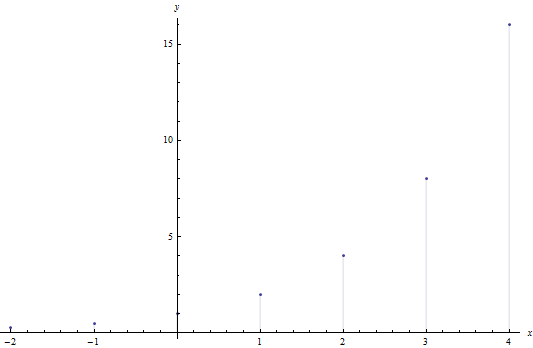
\includegraphics[width=0.7\textwidth]{imagens/2ax.png}
	\captionof{figure}{Alguns valores para $f(x)=2^x$}
	\label{fig:exeresol2ax}
\end{center}

Unindo os pontos:
\begin{center}

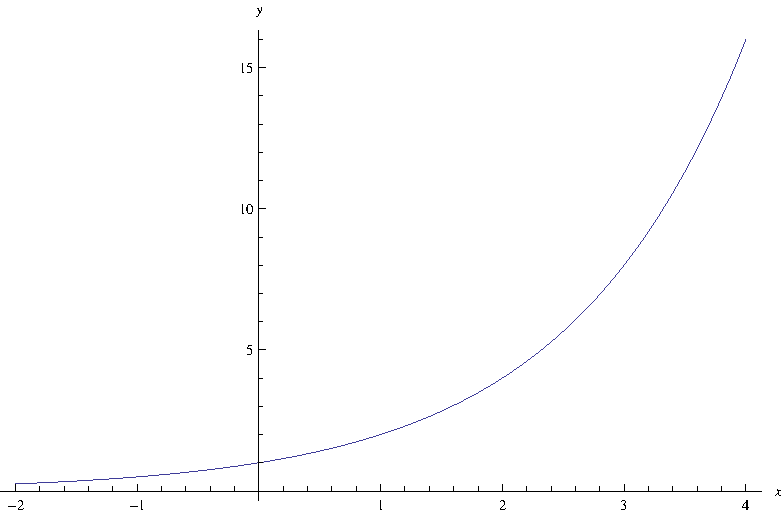
\includegraphics[width=0.7\textwidth]{imagens/2ax.pdf}
	\captionof{figure}{Gráfico de $f(x)=2^x$}
	\label{fig:exeresol2ax2}
\end{center}

\exem{Titulo}{Usando a mesma técnica, o gráfico de $f(x)=\frapar{1}{2}^x$ é }
\begin{center}

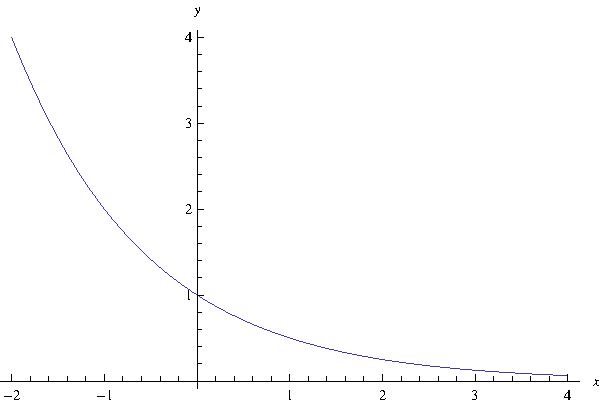
\includegraphics[width=0.7\textwidth]{imagens/05ax.pdf}
	\captionof{figure}{Gráfico de $f(x)=\frapar{1}{2}^x$}
	\label{fig:exemp05ax}
\end{center}


A função exponencial, conforme vimos nos gráficos anteriores, goza das seguintes propriedades:

\caixaprop{Seja $f$ uma função exponencial de base $a$, então
\begin{propriedade}\label{prop:exp_monotona} $f$ é crescente se $a>1$, é decrescente se $0<a<1$ e é constante se $a=1$
\end{propriedade}
\begin{propriedade}\label{prop:exp_injetora} $f$ é injetora se $a \ne 1$
\end{propriedade}
\begin{propriedade}\label{prop:exp_sobrejetora} $f$ é sobrejetora se $a \ne 1$
\end{propriedade}
\begin{propriedade}\label{prop:exp_bijetora} $f$ é bijetora e inversível se $a \ne 1$
\end{propriedade}
}

As demonstrações das propriedades estarão no apêndice.

\subsection{Equações e Inequações Exponenciais}
Equações Exponenciais são equações que apresentam incógnitas no expoente. Uma inequação exponencial é definida de forma análoga.
\exem{Titulo}{ $2^x = 0.5$ é uma equação exponencial enquanto $x^2 = 9$ não é.}

Nesse primeiro estudo de equações e inequações exponenciais, reduziremos as bases a um mesmo número e faremos uso das Propriedades \ref{prop:exp_bijetora} (para equações) e \ref{prop:exp_monotona} (para inequações).

\exem{Titulo}{Para resolvermos a equação $3^x = 9^4$ escreveremos todas as potências em uma base comum, nesse caso, $3$. Assim $3^x = (3^2)^4$ ou seja, $3^x= 3^8$. Pela Propriedade \ref{prop:exp_bijetora}, $x=8$.}
\begin{exeresol}
Resolva $4^x=2^6$
\begin{flushright}
\tiny[\textbf{Solução}: $x=3$ ]
\end{flushright}
\end{exeresol}
\exem{A técnica da Substituição}{Vamos ver uma técnica um pouco mais sofisticada. Vamos encontrar as soluções da equação $4^x -6. 2^x + 8=0$. O primeiro passo é escrevermos na mesma base.

O truque aqui é transformar $4^x = (2^2)^x = (2^x)^2$ e assim escrevemos $(2^x)^2 - 6.2^x + 8 =0$. Se substituirmos $t=2^x$ teremos $t^2 -6t + 8 = 0$, que é uma equação do segundo grau cujas raízes são $2$ e $4$. Assim teremos $t=2$ ou $t=4$. Se $t=2$ então $2^x=2$, de onde $x=1$ e se $t=4$ teremos $2^x=4$ e consequentemente $x=2$. Assim as soluções são $x=1$ ou $x=2$.}

\exem{Inequação exponencial}{A solução de $\frapar{1}{2}^x > 0.125$ pode ser encontrada escrevendo $0.125 = \frapar{1}{2}^3$. Assim $\frapar{1}{2}^x > \frapar{1}{2}^3$. Da Propriedade \ref{prop:exp_monotona}, temos que $x<3$ (lembre-se de que a exponencial é decrescente quando a base é menor que um).} 
\comecaexer
\subsection*{Exercícios}
\subsubsection{Exercícios Básicos}
\begin{exer} Simplifique
\end{exer}
\begin{enumerate}
\item $2^{\sqrt{2}}.2^{-\sqrt{2}}$
\item $(x^{\Pi})^{\Pi}$
\item $(\sqrt{2}^{\sqrt{2}})^{\sqrt{2}}$
\item $(\sqrt{5}^{\sqrt{2}-1})^{\sqrt{2}+1}$
\end{enumerate}
\begin{exer} Esboce o gráfico das seguintes funções definidas de $\R$ em $\R$
\end{exer}
\begin{enumerate}[a)]
\item $f(x) = 4^x$
\item $f(x) = 2^x+2$
\item $f(x) = - 2^x$
\item $f(x) = 5.2^x$
\end{enumerate}
\begin{exer} Resolva:
\begin{enumerate}[a)]
\item $2^x = 4$
\item $3^x = 1$
\item $4^x = 16^5$
\item $2^x = \sqrt[8]{64}$
\item $25^x = 5$
\item $2^x=0.5$
\item $2^x=0.125$
\item $4^x-2^x-2=0$
\item $5.2^{2x} - 4^{2x-\frac{1}{2}}-8=0$
\item $25^{\sqrt{x}} - 124.5^{\sqrt{x}} = 125$
\end{enumerate}
\end{exer}
\begin{exer} Resolva: $4^x + 6^x = 2.9^x$ (Dica: Divida ambos os lados por $9^x$)
\end{exer}
\begin{exer} Determine o conjunto solução:
\begin{enumerate}
\item $2^x>4$
\item $\frapar{1}{2}^x>256$
\item $0,0001 < 10^x < 0,001$
\item $\sqrt[3]{3}^x \leq \frac{1}{9}$
\item $4^x \geq 8$
\item $(3^x)^{2x-7}>\frac{1}{27}$
\item $\frapar{1}{2^x}^{3x+1}.4^{1+2x-x^2}\geq \frapar{1}{8}^{x-1}$
\end{enumerate}
\end{exer}
\begin{exer}
Encontre o conjunto solução de $x^{2x^2-9x+4}<1$ em \Rep. Dica: Considere isoladamente os casos $x=0$, $0<x<1$, $x=1$ e $x>1$.
\end{exer}
\begin{exer}
Resolver em $\Rep: x^{(x^2)}>x^{2x}$
\end{exer}
\subsubsection{Exercícios Avançados}
\begin{exer} Prove que existem dois números irracionais $a$ e $b$ tais que $a^b \in \Q$. Dica: Considere a expressão $(\sqrt{2}^{\sqrt{2}})^{\sqrt{2}}$
\end{exer}

\begin{exer}[PUC-Modificado] Qual é a soma das raízes de $5^{x^2-2x+1}=\frac{5625}{9}$?
\end{exer}

\begin{exer}[ITA] Determine o conjunto solução da equação $3^{2x} + 5^{2x} - 15^x=0$
\end{exer}

\begin{exer} Seja $a \in \R$ tal que $0<a<1$, resolva: $a^{2x}-(a+a^2).a^x+a^3<0$
\end{exer}
\begin{exer}[IME] Resolva o sistema
$ \left\{
\begin{array}{ll}
\displaystyle x^y=y^x \\
\displaystyle x^3=y^5\\
\displaystyle x>0
\end{array}
\right.
$
\end{exer}
\terminaexer